\subsection{Celda de carga}
La celda de carga es un dispositivo capaz de traducir la fuerza aplicada sobre ella  en una señal eléctrica medible. En su interior están compuestas por galgas extensiométricas, una matriz de resistencias conectadas en forma de puente de Wheatstone, se observa en la \autoref{fig:celda}.
\begin{figure}[H]
    \centering
    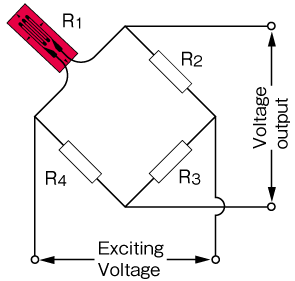
\includegraphics[width=0.7\textwidth]{Secciones/marcoTeorico/media/celda.png}
    \caption{Celda de carga}
    \label{fig:celda}
\end{figure}
Donde la tensión de salida es:
\begin{equation}\label{eq:VoCelda}
    V_{out} = V_{in} \left(\frac{R1\cdot R3 - R2\cdot R4 }{(R1+R2)(R3+R4)}\right)
\end{equation}
Que cada vez que se coloca un elemento sobre ella, el bloque de alumino se deforma y en consecuencia las galgas se deformaran, variando así su resistencia eléctrica en proporción a la deformación producida. Esta variación será lineal siempre y cuando se trabaje en la zona lineal del material que conforma la galga de manera que la deformación que se produzca sea perfectamente elástica, es decir que la galga tenga la capacidad de volver a su forma original luego de la perturbación (ley de Hook).
\begin{figure}[H]
    \centering
    \begin{subfigure}[b]{0.49\textwidth}
        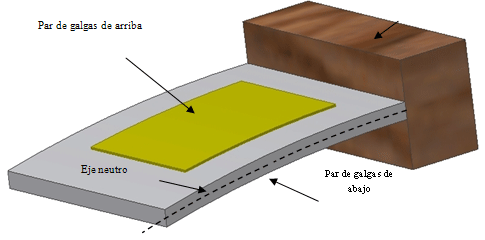
\includegraphics[width=\textwidth]{Secciones/marcoTeorico/media/galga1.png}
        \caption{}
        \label{fig:f1}
    \end{subfigure}
        \begin{subfigure}[b]{0.49\textwidth}
        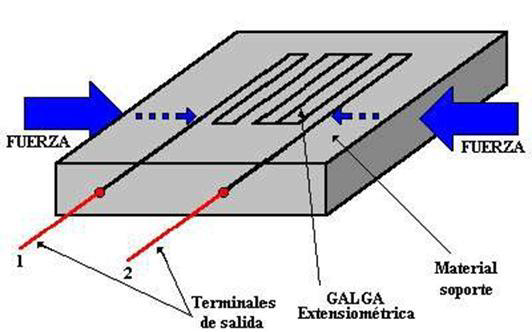
\includegraphics[width=\textwidth]{Secciones/marcoTeorico/media/galga2.png}
        \caption{}
        \label{fig:f2}
    \end{subfigure}
    \caption{}
    \label{fig:galga}
\end{figure}
\subsection{Amplificación y Acondicionamiento}
Como la celda de carga emitirá una señal eléctrica de tipo diferencial que es proporcional a la deformación producida por el peso. Debido a las limitaciones de los ADC, esta señal para poder ser digitalizada, posteriormente procesada y mostrada al operador de la balanza deberá ser amplificada en un rango que cumpla con los requerimientos del conversor.
\\Debido a las exigencias de medida que imponen los sensores, se ha decidido conformar un amplificador de instrumentación a través de amplificadores operacionales individuales \autoref{fig:aoInstrument}. Estos tienen la particularidad de tener alta impedancia de entrada, baja impedancia de salida, ganancia variable, estable lineal y alta CMRR (hecho que nos favorece especialmente ya que nuestra señal de entrada es diferencial pura y queremos eliminar lo máximo posible el modo común).

\begin{figure}[H]
    \centering
    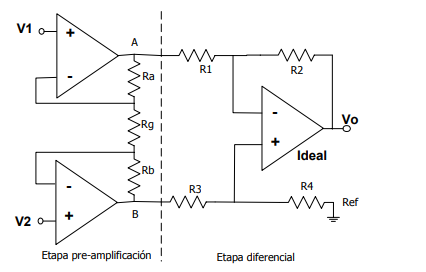
\includegraphics[width=0.7\textwidth]{Secciones/marcoTeorico/media/aoInstrument.png}
    \caption{Configuración del amplificador de instrumentación}
    \label{fig:aoInstrument}
\end{figure}
Donde V1 que será la tensión máxima que tenemos en el puente $(Vcc+ \Delta v)$ y V2 la tensión mínima$(Vcc- \Delta v)$.

La etapa de pre-amplificación aumenta la impedancia de entrada del conjunto y hace que se cancelen entre sí los posibles errores, sólo tendremos errores por características constitutivas propias de los amplificadores. Una buena forma de disminuirlos es utilizar una misma pastilla para desarrollar el amplificador de instrumentación ya que si todos los operacionales pertenecen a la misma pastilla sus errores tienden a ser iguales.

Profundizando sobre esto, analizaremos la salida en función de las entradas V2 y V1:
\\Obteniendo la tension en los punto A y B:
\begin{equation*}
    \begin{split}
        \frac{VA-V1}{RA} &= \frac{V1-V2}{RG} \Rightarrow
        VA = V1 \left(\frac{RA}{RG} + 1\right) - \left(\frac{RA}{RG}\right)V2\\
        \frac{V1-V2}{RG} &= \frac{V2-VB}{RB} \Rightarrow
        VB = V2 \left(\frac{RB}{RG} + 1\right) - \left(\frac{RB}{RG}\right)V1\\
    \end{split}
\end{equation*}
Restando ambas expresiones:
\begin{equation*}
    VB-VA = V2 -V1 \left(\frac{RA+RB}{RG} + 1 \right)
\end{equation*}
Donde el termino entre paréntesis representa la ganancia de la etapa pre-amplificadora, variando RG podemos variar dicha ganancia.
\\Analizando la etapa diferencial:
\begin{equation*}
    V o=-\frac{R 2}{R 1} V A+\left(1+\frac{R 2}{R 1}\right)\left(\frac{R 4}{R 3+R 4}\right) V B
\end{equation*}
Reemplazando VA, VB y considerando que $Vd=VB-VA$ y $Vcm=\frac{VA+VB}{2}$
\begin{equation}\label{eq:Vo}
    V o=-V d\left(\frac{1+\frac{R 2}{R 1}}{1+\frac{R 3}{R 4}}\left(\frac{1}{2}+\frac{R B}{R G}\right)+\frac{R 2}{R 1}\left(\frac{1}{2}+\frac{R A}{R G}\right)\right)+V c m\left(\frac{1-\frac{R 2 R 3}{R 1 R 4}}{1+\frac{R 3}{R 4}}\right)
\end{equation}
De la ecuación \autoref{eq:Vo} podemos notar que:
\begin{itemize}
    \item La ganancia en modo comun sera: 
    \begin{equation*}
        Ac = \left(\frac{1-\frac{R 2 R 3}{R 1 R 4}}{1+\frac{R 3}{R 4}}\right)
    \end{equation*}
    y deseamos que sea nula para ello \begin{equation*}
        \left(\frac{1-\frac{R 2 R 3}{R 1 R 4}}{1+\frac{R 3}{R 4}}\right) = 0 \Rightarrow \frac{R2}{R1} = \frac{R4}{R5}
    \end{equation*}
    \item Tomando: \begin{equation*}
        RB = RA \Rightarrow Ad = \frac{R2}{R1}\left(1+\frac{2RA}{RB}\right)
    \end{equation*}
    \item Si tenemos en cuenta los dos puntos anteriores, podríamos considerar que a priori la $RRMC \Rightarrow \infty$ valor deseado.
\end{itemize}